\documentclass[10pt,b5paper, twocolumn]{ltjsarticle}
\usepackage[paper=b5j, bmargin=100pt]{geometry}
\usepackage{luatexja}
\usepackage[utf8]{inputenc}
\usepackage{amsmath}
\usepackage{amssymb}
\usepackage{mathtools}
\usepackage{leadsheets}
\makeatletter
\let\meterC\relax
\makeatother
\usepackage{musicography}
\usepackage{luatexja-ruby} 
\usepackage{wrapfig}
\usepackage{caption}
\usepackage{makecell}
\usepackage{dashrule}
\usepackage{graphicx}
\usepackage{xcolor}
\graphicspath{ {./resources/} }
\usepackage{hyperref}
\usepackage{subcaption}
\usepackage[document]{ragged2e}

\setchords{
    major-seven = \textsuperscript{M7},
    major-nine = \textsuperscript{M9}
}

\renewcommand*\contentsname{目次}
\renewcommand{\figureautorefname}{図}
\renewcommand{\tableautorefname}{表}
\setlength{\RaggedRightParindent}{\parindent}
\setlength{\abovecaptionskip}{0pt plus 3pt minus 2pt}
\RaggedRight
\pagenumbering{roman}
\addtocounter{page}{1}
\setcounter{tocdepth}{2}

\title{\huge{コードオタクが語る東方楽曲分析}  \vspace{3pt} \hrule \vspace{3pt} {\large{第四弾　風神少女と妖怪の山の関連性}}}
\author{{Metalloid.}}
\date{{2026-10}}

\newcommand{\wc}{\writechord}
\NewDocumentCommand{\sd}{}{\musDegree}
\definecolor{bgc}{RGB}{255, 245, 206}


\begin{document}
\maketitle

%{\huge{コードオタクが語る東方楽曲分析}}
%\vspace{3pt}
%\hrule
%\vspace{3pt}
%\rightline{\large{第三弾　風神少女から垣間見る\ruby{調}{キー}からの逸脱}}
%\vspace{12pt} \rightline{Metalloid.} \rightline{10/2025}

\tableofcontents

\vspace{12pt}
\hrule
\vspace{12pt}
\section{まえがき及びテーマ}
どうも、Metalloid.です。今回は射命丸文のテーマ曲たちー\textbf{「風神少女」および「妖怪の山 ~ Mysterious Mountain」の間にどのような関連性があるのか}を和声的観点から考えてみようと思います。前回23号で寄稿した第三弾ー「風神少女」の分析はかなり本格的な記事になっていたので、今回は少し緩めの内容にするとともに、二段組形式を試運転しようなどと考えています。二段組の方が綺麗に収まった場合今後も二段組を活用していくかもしれません。\par
\vspace{10pt}
\begin{figure}[h]
    \centering
    
\includegraphics[width=0.3\linewidth]{qr.png} 
    \label{fig:qr}
    \caption*{音声コンテンツ}
\end{figure}
前回同様、本稿の譜例に対応する簡単な音声ファイルを準備しているので、是非ご活用ください～
\par
%\vspace{5pt}
% 最後に、色んな層の人に楽しんで頂けるように、場所によっては高度な内容にも触れています。\textbf{難しいと感じる節があれば読み飛ばすのがオススメです。}
\section{分析}
\subsection{両曲の鳥瞰図}
まず、両方の曲の構成を大きく俯瞰していきましょう。
\begin{figure}[h]
    \centering 
    \begin{subfigure}{0.4\linewidth}
        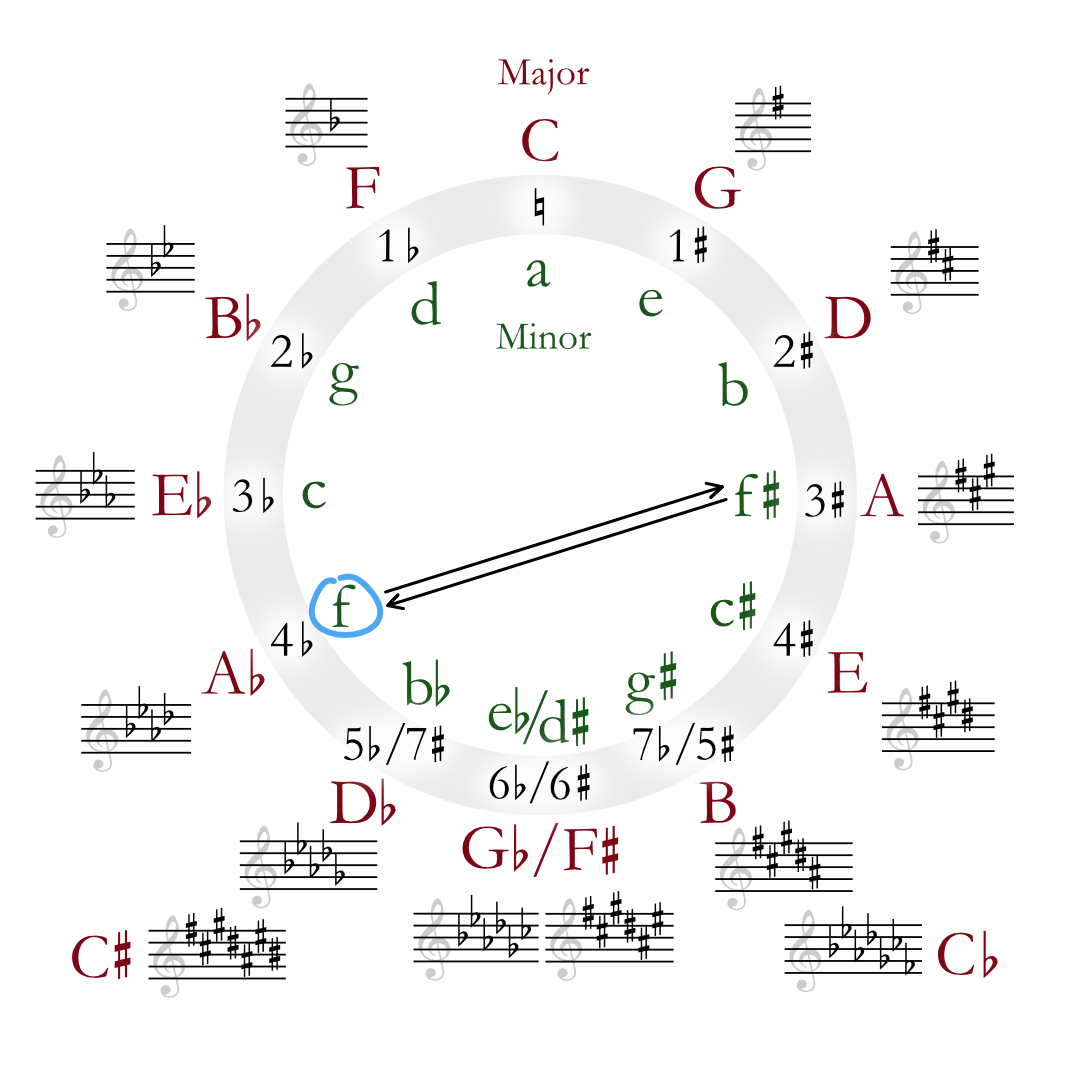
\includegraphics[width=\textwidth]{windKeyOverview.png} 
        \label{fig:windKeyOverview}
        \caption{風神少女}
    \end{subfigure}
    \begin{subfigure}{0.4\linewidth}
        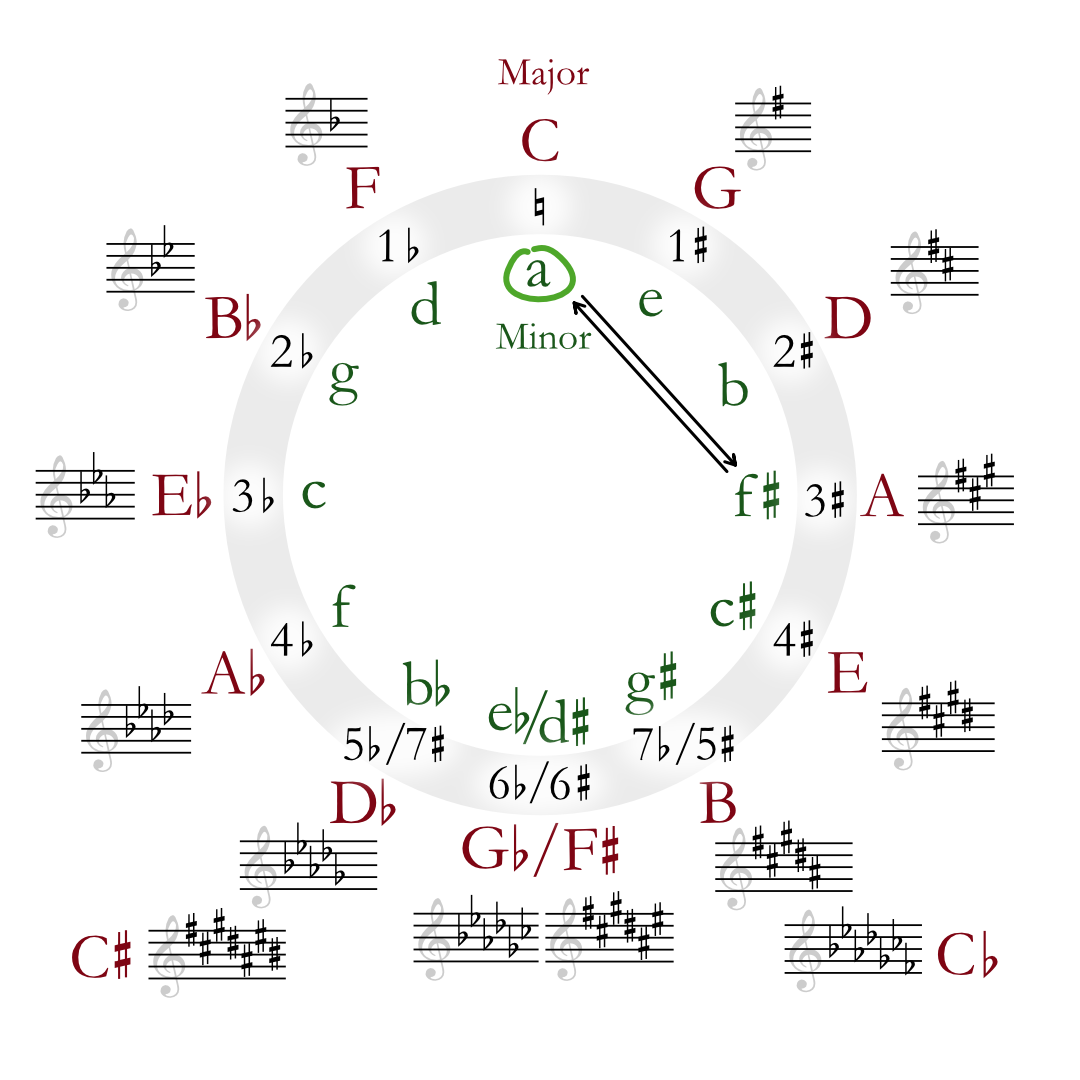
\includegraphics[width=\textwidth]{mountainKeyOverview.png} 
        \label{fig:mountainKeyOverview}
        \caption{妖怪の山の転調鳥瞰図}
    \end{subfigure}
    \label{fig:keyOverview}
    \caption{転調鳥瞰図\cite{circleFifths}}
\end{figure}

\subsection{風神少女の特徴}

\subsection{妖怪の山の特徴}

\subsection{ドリアンスケールと射命丸文}

\subsection{まとめ}

\begin{figure}[h]
    \centering
   % \vspace{-60pt}
    \fcolorbox{black}{bgc}{
        \begin{minipage}{\linewidth}
        \textbf{アンダルシア進行} \\ ローマ数字で記述するなら、\wc{i bVII bVI V}。スペインのフラメンコ音楽が起源である。学者によっては、歴史的文脈に於いてこの進行をフリジアン音階における\wc{iv bIII bII I}と評価し、最後のコードをトニックとして解釈する者もいる。今回はそのような用法ではなく、一つ目のコードがトニックとなっている。
        \end{minipage}
    }
\end{figure}

\section{付録}

\subsection{本稿における表記法と思想}
音楽理論を扱う世のマテリアルでは表記（と流派）が異なることも多いので、本稿で使用する表記とコードの解釈について追記します。特に、東方は短調ベースで書かれることが多く、臨時記号も多用するので、それに適応した表記として、長調としての表記・分析より短調としての表記や分析を行うことが多いと思います。\par
具体的に、コードのルートに対する度数とスケールに対する度数を区別するため、後者をアクセント付きの数字で表記していきます。（\autoref{fig:scales}）\par
\begin{itemize}
    \item  長音階に関しては \sd{1} \sd{2} \sd{3} \sd{4} \sd{5} \sd{6} \sd{7} と表記
    \item 自然短音階は \sd{1} \sd{2} \fl \sd{3} \sd{4} \sd{5} \fl \sd{6} \fl \sd{7} と表記
    \item その上で、臨時記号をその都度用いる（例: 和声短音階は \sd{1} \sd{2} \fl \sd{3} \sd{4} \sd{5} \fl \sd{6} \na \sd{7} ）
\end{itemize}

\begin{figure}
    \centering
    \begin{subfigure}{0.4\textwidth}
        \centering
        
\includegraphics[width=\linewidth]{appendix/major scale.png}
        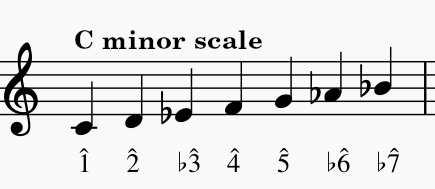
\includegraphics[width=\linewidth]{appendix/minor scale.png}
        \caption{長音階、短音階}
        \label{fig:scales}
    \end{subfigure}
    \begin{subfigure}{0.4\textwidth}
        \centering
        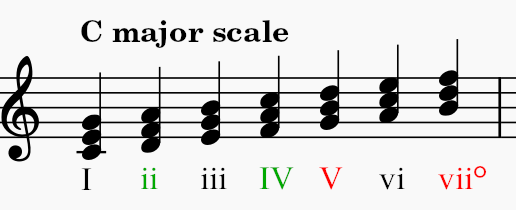
\includegraphics[width=\linewidth]{appendix/major scale chords.png}
        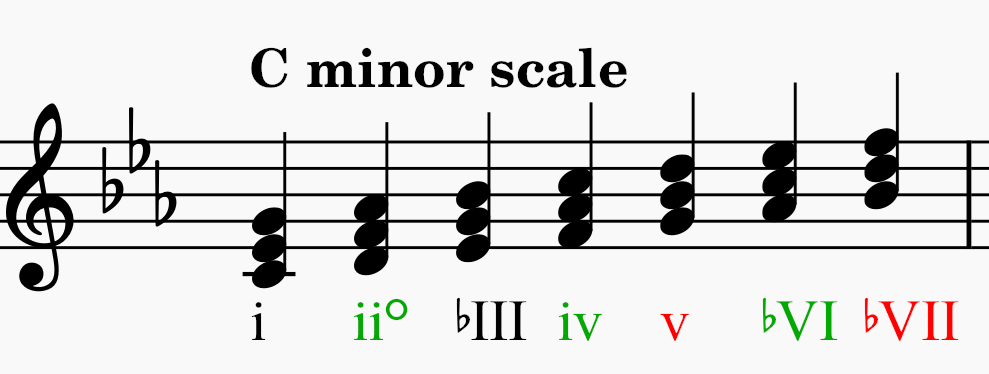
\includegraphics[width=\linewidth]{appendix/minor scale chords.png}
        \caption{長音階、短音階のダイアトニックコード}
        \label{fig:diatonicChords}  
    \end{subfigure}
    \caption{本稿での表記}
    \label{fig:notation}
\end{figure}

また、コードのローマ数字表記に関して、メジャーコードとマイナーコードの表記法を区別します。（\autoref{fig:diatonicChords}）
\begin{itemize}
    \item メジャーコードは大文字
    \item マイナーコードは小文字
    \item コードエクステは重要であると判断した場合に表記
\end{itemize}
続いてダイアトニックコードの役割ですが、ダイアトニックコードの役割は教材・ソースによって割れることも多々あるので予めここで本稿においての考えを断っておきます。（\autoref{tab:diatonicFunctions}）
\begin{itemize}
    \item 長調
    \begin{itemize}
        \item \writechord{I}, \writechord{iii}, \writechord{vi}はトニック役  
        \item \writechord{V}, \writechord{viio}はドミナント役
        \item \writechord{ii}, \writechord{IV}はプレドミナント役   
    \end{itemize}
    \item 短調
    \begin{itemize}
        \item \writechord{i}, \writechord{bIII}, \writechord{vi}はトニック役  
        \item \writechord{v}, \writechord{bVII}はドミナント役
        \item \writechord{iio}, \writechord{iv}, \writechord{bVI}はプレドミナント役   
    \end{itemize}
\end{itemize}

\begin{table}
    \centering
    \caption{コードの役割}
    \begin{tabular}{|c|c|c|c|}\hline
        調 & トニック & ドミナント & プレドミナント \\\hline
        長調 & \makecell{\writechord{I} \\ \wc{iii} \\ \wc{vi}} & \makecell{\wc{V} \\ \writechord{viio}} & \makecell{\wc{IV} \\ \wc{ii}} \\
        短調 & \makecell{\writechord{i} \\ \wc{bIII}} & \makecell{\wc{v} \\ \writechord{bVII}} & \makecell{\wc{iv} \\ \writechord{bVI} \\ \wc{iio}} \\ \hline
    \end{tabular}
    \label{tab:diatonicFunctions}
\end{table}

\bibliographystyle{plain}
% \bibliographystyle{aipnum-cp}%
\bibliography{references}

\end{document}
